\section{Archive Behaviour}
This section describes the design and behaviour of archiving a MARS complete project. Table \ref{table:preconditionsArchive} presents the preconditions with its 
description which are required for the archiving process to occur. 

\begin{table}[H]
    \centering
    \begin{tabular}{|p{3cm}|p{11cm}|}
        \hline
            \textbf{Preconditions}  & \textbf{Description}\\
        \hline
            Mark resources & 
            The resources must be marked using the MARS marking service. This is necessary to prevent the resources to be modified during the archive process. \\
        \hline
            Get Metadata for the project
            & The metadata contains all necessary information about the files. The scenarios, files and the result configuration depends on these metadata getting 
            the respective data.\\  
        \hline
            Get Simulation runs & The simulation runs contains the simulation id which is required to archive the correct simulation id. This dependency
            with simulation run makes is necessary that the simulation runs are obtained before archiving simulation results. \\
        \hline
    \end{tabular}
    \caption{Preconditions required for an archive process}
    \label{table:preconditionsArchive}     
\end{table}    

\subsection{Data format}
The first step for archiving is to decide the file format to store the archived data. This is
considered to be the initial step because it determines how the data can be accessed and whether it meets
the criteria mentioned in Section \ref{section:functionalReq}.

\par
The following file systems are analzyed for this thesis:
\begin{enumerate}
    \item Web Archive (WARC file format)\footnote{https://www.iso.org/standard/44717.html}
    \item Hierarchical data format 5 (HDF5)\footnote{https://support.hdfgroup.org/HDF5/whatishdf5.html}
\end{enumerate}

HDFS\footnote{https://hortonworks.com/apache/hdfs/} is a very popular file system used to store big data in an efficient and fast manner. 
Although, having its benefits it was not compared because of the complexity to configure a Hadoop server for the MARS system. This is mentioned in this thesis since it would be
a point of interest in the future to add this file format in the Archive service to utilize the benefits that it provides.

\subsubsection{HDF5}
HDF5 is a file format for storing and managing data which has support for various data types designed for
efficient I/O which has the capability to support big data. This file format is portable which helps to speed
up the application development. An HDF5 file is an abstract data container which includes building blocks for data organization. This file
system can hold a variety of heterogeneous objects \cite{Savic2007}. 

\subsubsection{WARC}
The WARC (Web Archive) file format is used to archive web files by concatenating multiple resource records
(data objects), each consisting of a set of simple text headers and an arbitrary data block into one long file.
This file format can be used to store different kinds of web crawl data with its metadata. It is widely used
 to archive data from the World wide web i.e. images, texts, html \cite{WARC}.

 \begin{table}[H]
    \centering
    \begin{tabular}{|p{7.5cm}|p{7.5cm}|}
        \hline
            \textbf{HDF5}  & \textbf{WARC}\\
        \hline
            It is used mostly for scientific purposes (Efficient
            for simulation data \cite[p.~11]{Savic2007}. & 
            Ability to store both the payload content and control information from mainstream Internet application layer protocols, such as
            HTTP, DNS, and FTP. \\
        \hline
            It enables efficient data storage on lookup.
            &  
            Support for data compression and maintenance of
             data record integrity.\\
        \hline
        Can be utilized with different programming languages with fast access (i.e. java, matlab, python etc.) &  
                Ability to be extended without disruption
                to existing functionality.\\
        \hline
        Separates raw data with its metadata. & Support handling of overly long records by. \\        
        \hline
        
        \hline
    \end{tabular}
    \caption{Comparison between HDF5 and WARC}
    \label{table:Hdf5vsWARC}     
\end{table} 

\subsubsection{Conclusion}
    The two file formats are very powerful in their own domain and it can be utilized to archive a file very effectively. After careful consideration,  
    it seems so that both of the file formats are not suitable for the archive and retrieve process. 

    HDF5 file format is not suitable for our use case because this format is highly optimized to work with
    numeric data for fast access and storing variable length string is inefficient as it creates a large overhead to store them. 
    Additionally, it also requires additionally 3rd party application for viewing and extracting its data which 
    adds more complexity for the user if one just wants to download the archive and analyze it. 

    The WARC is found not suitable because the WARC cannot handle file sizes more than 1GB properly \cite[Appendix B]{WARC}. 
    In contrast to MARS simulation results where a single results could be larger than 1GB. This would results in scalability issues in the future. To 
    avoid this circumstance this file format was also excluded.

    Lastly, the file format for archive is planned to be json for the metadata files i.e. simulation runs, simulation plans, scenarios and, result configuration and 
    the simulation results would be stored as a gzip file. All the project resources will be packed inside a folder in the Synology (See Figure \ref{fig:synology})
     which is easily accessible via the MARS network.
    The folder can be downloaded as a zip file as the synology provides an graphical UI to work with.   

\begin{figure}[H]
    \centering 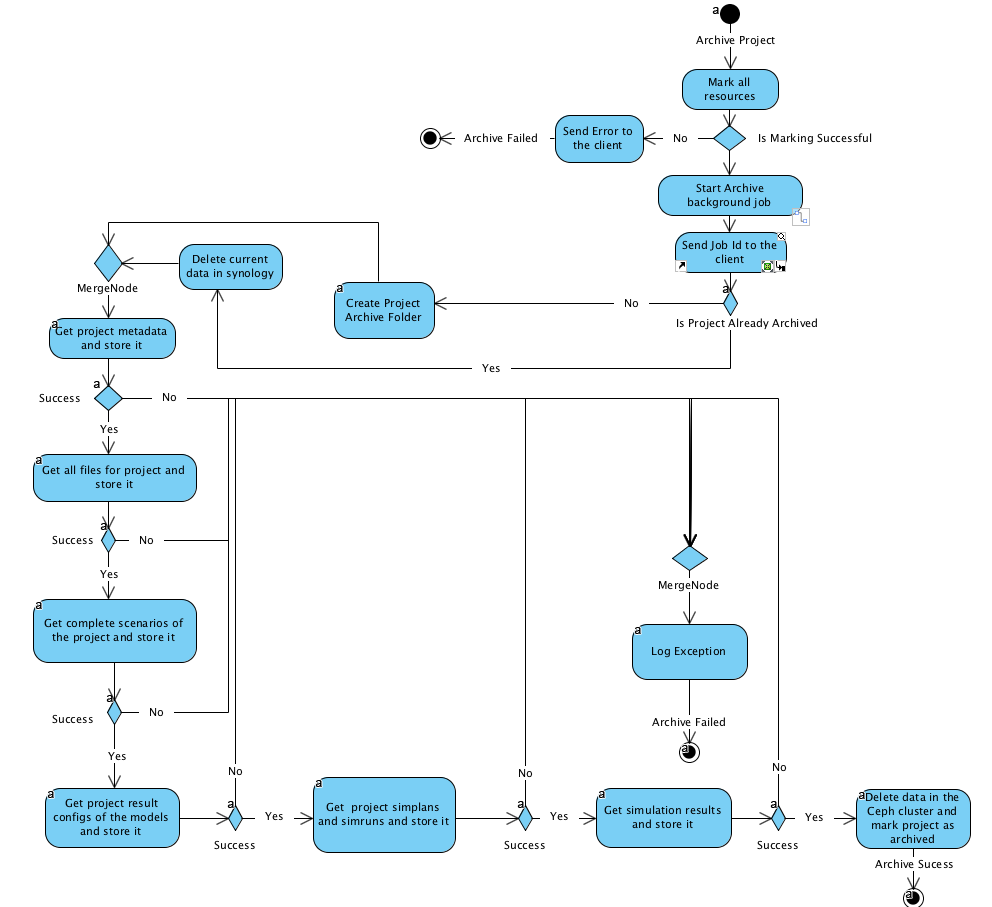
\includegraphics[scale=0.45]{grafiken/archiveActivity.png}
    \caption{Activity Diagram of MARS project Archive process}
    \label{fig:archiveActivity}
\end{figure}

Figure \ref{fig:archiveActivity} illustrates an activity diagram of archiving an entire archive process. As mentioned in Table \ref{table:preconditionsArchive},
marking the resources for the project for the archive service is the first requirement needed to start the process. If the project resources are marked successfully
than the archive would be initialized as a background job and the job id would be send to the client. In case the marking would fail the error message will be 
sent to the client and the archive process will halt. The archiving process is visioned to be an background job due to the fact that a single process could take
a long period of time and would block the server for additional requests. Following the successful job creation action, the process checks if an archive already
exists. A check for an existing project is made to ensure that if the archive process failed caused by an transient error, the incomplete data can be removed. After
the archive folder creation the metadata, files, scenarios, result configurations, simulation plans, simulation runs and the simulation results are retrieved respectively.
After a successful archive process the  resources are deleted from the Ceph cluster. Lastly, in case of some failures during archiving the exception will be logged 
which can be later analyzed for maintenance.

\begin{figure}[H]
    \centering 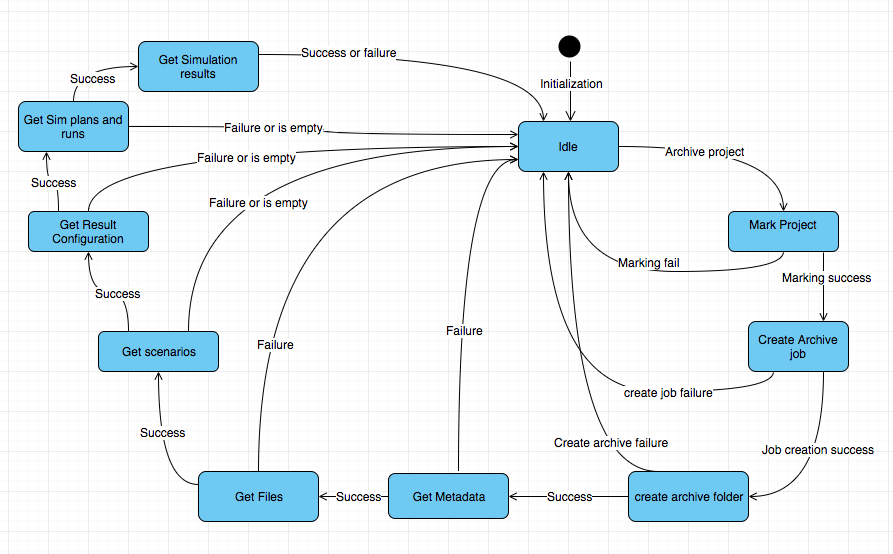
\includegraphics[scale=0.45]{grafiken/stateArchive.png}
    \caption{State Diagram of MARS project Archive process considering empty states}
    \label{fig:stateArchive}
\end{figure}

Figure \ref{fig:stateArchive} illustrates the transitions that can occur during the archive process. The idle refers to the state where no archive process
is being executed. Additionally, the state digram also considers
how the state would change if one of the resources is empty. In the case of an empty resource (e.g. no scenarios available for the project) the archive
process stops gracefully without any errors goes to the idle state. 

 